% AERO2711 progress report -- LaTeX version.
% Compile with pdfLaTeX (Overleaf default) or tectonic. Figures are in figs/.
\documentclass[12pt,a4paper]{article}
\usepackage[utf8]{inputenc}
\usepackage[T1]{fontenc}
\usepackage{amsmath,amssymb}
\usepackage{newtxtext,newtxmath}
\usepackage[a4paper,left=3cm,right=2cm,top=2.54cm,bottom=2.54cm]{geometry}
\usepackage{setspace}
\onehalfspacing
\usepackage{graphicx}
\usepackage{float}
\usepackage{array,booktabs}
\usepackage{enumitem}
\usepackage[table]{xcolor}
\usepackage{textcomp}
\usepackage{listings}
\usepackage{cite}
\usepackage[skip=6pt]{caption}
\usepackage[hidelinks]{hyperref}
\lstset{basicstyle=\ttfamily\footnotesize,breaklines=true,columns=fullflexible}
\setlist{itemsep=2pt,topsep=4pt}
\setlength{\parskip}{4pt}
\newcommand{\ph}[1]{\colorbox{yellow}{#1}}

\begin{document}

\begin{titlepage}
  \centering
  \vspace*{3cm}
  {\large\color{gray} AERO2711 Research Project --- Progress Report\par}
  \vspace{1cm}
  {\LARGE\bfseries Visual Active Tracking of Manoeuvring Targets\\ under Occlusion\par}
  \vspace{0.6cm}
  {\large\itshape Map-constrained prediction and edge-aiming blind-phase control\\ for a drone-mounted camera\par}
  \vspace{3cm}
  \textbf{Student:} Yujie Ding (SID: 530675228)\par
  \textbf{Supervisor:} Dr Zihao Wang\par
  \vspace{1.5cm}
  The University of Sydney\par
\end{titlepage}

\clearpage
\section*{Abstract}
\addcontentsline{toc}{section}{Abstract}
Visual active tracking (VAT) systems steer a camera to keep a person in view. When a wall or another obstacle hides the person, the tracker has to judge where the person will reappear, so that it can follow them again quickly. Current systems, including the recent OA-VAT framework, use a constant-velocity (CV) Kalman filter for this and are evaluated on targets that walk at near-constant speed. This project studies targets that speed up or slow down while they are hidden.

On a calibrated occlusion benchmark in Unreal Engine (an L-shaped corner), upgrading the motion model from CV to constant acceleration (CA) gave no significant gain. Most of the error came from how the filter is used during the occlusion. Partially occluded measurements corrupt its last estimate, and its blind-phase prediction drifts into walls. A reactive controller that steers toward this prediction then carries the error into the camera motion. This project tests a set of changes that use a map of the scene. It combines a \textbf{map-constrained Kalman filter (MC-KF)}, which repairs partially occluded measurements and moves the blind-phase prediction back into the free space of the map, with \textbf{edge-aiming blind-phase control}: while the target is hidden, the camera turns toward the edge of the obstacle instead of toward the filter's prediction and speeds up to full speed. Since no planner is used, in practice the camera slides along the wall toward the corner. The camera has inertia, and a braking-distance safety layer, used in every configuration, keeps it clear of walls. Compared with the CV Kalman filter released with OA-VAT, run with the same ideal detector, controller and safety layer on random target motion, the system reduces the re-acquisition error from 111 px to 21 px (better on 34 of 36 paired seeds), with success rate 1.00 and no wall collisions.
With the map projection in place, a CA filter is worse than CV, because its acceleration term and the projection correct the same lag; this suggests that, in this setting, the improvement comes from how the filter is used rather than from the motion model.

\clearpage
\tableofcontents
\clearpage
\section{Background and Motivation}
% --- Paragraph 1: the task and the problem ---
Small drones are increasingly used to follow a person automatically, for example for filming, inspection or search and rescue.
This task is called \emph{visual active tracking} (VAT): unlike a normal tracker, which only marks the person in a video, an active tracker also moves the camera to keep the person in view at a suitable distance \cite{r1,r2}.
Indoors and in cities, a common reason for failure is occlusion: a wall, a building or another obstacle hides the person, and the tracker must decide where to look and where to fly without seeing them.
The goal is to find the person again quickly once they reappear.

% --- Paragraph 2: how trackers handle this today ---
Most VAT systems bridge this gap with a Kalman filter that uses a constant-velocity (CV) model.
``Constant velocity'' is the filter's assumption, not a description of the person: the filter moves the last known position forward as if speed and direction stayed the same, and treats any difference as noise.

% --- Paragraph 3: the gap and what motivated this project ---
The recent OA-VAT system \cite{r3} uses such a filter, and the people in its tests walk at an almost constant speed, so this assumption is rarely tested.
Real people, however, often speed up, stop or turn once they are out of sight; this is the usual way to escape a follower \cite{r4}.
Two small tests made while reproducing OA-VAT pointed to this problem: its tracking score dropped when the person accelerated, and at corners its predictor did no better than using no predictor at all (Section 6.1).
This project asks what goes wrong when a person changes speed while hidden, and how the tracker should handle it so that the person is found again quickly.

% --- Paragraph 4: first answer, the real cause, and the approach ---
The obvious answer is a better motion model, such as a constant-acceleration (CA) filter, which can follow a person who is speeding up.
Neither model matches the people here exactly, because they change speed at random moments, sometimes while they are hidden.
In this project the CA filter gave no significant gain.
The larger errors come from three other sources.
First, while an obstacle hides part of the person, the detected box is cut off, so the filter is given a wrong position.
Second, while the person is fully hidden, the prediction can drift into a wall, where no person can be.
Third, if the camera turns toward this wrong prediction, the error goes straight into where the camera looks and flies.
Since the layout of walls and corridors is usually known or can be mapped, this project uses a map of the surroundings to correct the filter and to guide the camera, in a way that works with any motion model.
The method is developed and tested on an L-shaped corner, the simplest layout that produces a repeatable occlusion.

\section{Literature Survey}
\subsection{Visual active tracking}
Luo et al. \cite{r1,r2} trained a single neural network with reinforcement learning to turn camera images directly into camera movements, using virtual worlds built with UnrealCV \cite{r5}.
Later work made this approach more robust: AD-VAT \cite{r6} trains the tracker against a target that learns to escape, \cite{r7} adds people who look similar to the target, RSPT \cite{r8} rebuilds the surroundings and predicts the target's path so that the tracker works in new scenes, and \cite{r9} uses large pre-trained vision models with reinforcement learning from recorded data.
In all of these methods, the handling of occlusion is hidden inside the network's memory, so when tracking fails it is hard to tell whether the prediction or the control was wrong.
OA-VAT \cite{r3} is instead built from separate modules.
It finds and identifies the person with YOLOE \cite{r10}, DINOv3 features \cite{r11} and ORTrack \cite{r12}.
When the person is lost, it stops the camera, predicts where the person has gone with a Kalman filter that weighs each measurement by the detector's confidence, searches there, and hands over to a diffusion-policy planner \cite{r13} if the person is still not found.
This project reuses its Kalman filter, evaluation protocol and simulator (Section 5.1), but not its tracking pipeline.

\subsection{Motion models and occlusion in tracking}
The Kalman filter \cite{r14} is optimal when the motion model matches the target. For targets that do not follow a fixed model, the tracking literature offers the Singer acceleration model \cite{r15}, a family of dynamic models surveyed by Li and Jilkov \cite{r16}, and the Interacting Multiple Model (IMM) estimator \cite{r17}, the standard tool in radar and aerospace tracking \cite{r18}. All of these assume a steady stream of measurements. During a long occlusion there are no updates, and every model reduces to open-loop extrapolation from the estimate at the moment the target disappeared.

In computer vision, the SORT family \cite{r19,r20,r21} runs a CV Kalman filter on the bounding box to bridge missed detections. OC-SORT \cite{r22} shows that a filter coasting through occlusion builds up error, mainly through its noisy velocity estimate, and corrects the filter \emph{after} the target is found again. ORTrack \cite{r12} makes the appearance model robust to partial occlusion.
A related, well-known issue is that a box cut off by an obstacle has its centre shifted toward the visible side, just before the target disappears.
Trackers usually handle this by trusting such measurements less, as OA-VAT and StrongSORT \cite{strongsort} do by scaling the measurement noise with detector confidence, or by training detectors to predict the full extent of a partly hidden object \cite{amodal}.
When the layout of the scene is known, a simple complementary option is to use it directly; this project explores rebuilding the box centre from its visible edge, with the map indicating which side is cut off.

\subsection{Scene-aware prediction and constrained estimation}
Human trajectory prediction has moved to learned models that take the surroundings into account \cite{r23}, such as Social LSTM \cite{r24} and Trajectron++ \cite{r25}.
Kitani et al. \cite{r26} showed that knowing where a person \emph{can} walk strongly narrows down long-range forecasts.
These predictors are mostly evaluated offline on recorded trajectories, rather than inside a tracking loop where the camera itself moves.
In estimation theory, known physical limits can be added to a Kalman filter; this is called \emph{state-constrained Kalman filtering} \cite{r27}.
The simplest method, estimate projection, moves an estimate that falls outside the allowed region to the nearest point inside it.
The MC-KF in this project applies this idea, with the free space in a map of the surroundings (here, the corridor) as the allowed region, after converting the image position to a floor position.

\subsection{Aerial target following among obstacles}
Model-based aerial trackers plan drone trajectories with explicit collision and visibility terms \cite{r28,r29,r30}. Fast-Tracker \cite{r31} and Elastic Tracker \cite{r32} track agile targets in clutter using a map of the environment \cite{r33} and a kinematic prediction of the target. They are designed to \emph{prevent} occlusion, and they assume a metric map and a 3D target state. Collision safety is often enforced with control barrier functions \cite{r34}, which change a nominal command as little as possible. The safety layer used here follows the same idea at velocity level, and never changes the heading.

\subsection{Summary}
In short, most trackers bridge occlusion with a constant-velocity filter, and common VAT benchmarks rarely test targets that change speed while hidden.
Known scene layouts are widely used in trajectory prediction and aerial planning, but less often inside the estimator of an active tracker.
This project therefore tests, in a small simulation study, whether a map of the surroundings can improve re-acquisition after occlusion when the target changes speed.

\section{Problem Statement}
\textbf{In a simulated drone tracking system, how can the processing of measurements, the prediction and the camera's motion during occlusion be arranged, using a map of the surroundings, so that a person who changes speed while hidden behind an obstacle is found again quickly and without collisions?}

The design target is a re-acquisition error below about 30 px, with success rate 1.00 and zero wall contacts, for targets that move along random routes at random speeds.

\subsection{Work to date}
\begin{enumerate}[label=\textbf{C\arabic*.}]
  \item \textbf{Map-constrained Kalman filter (MC-KF).} A standard box-space Kalman filter with two map-based steps: repairing partially occluded measurements, and moving the blind-phase prediction back into the free space of the map. It is used with the CV model (Section 6.4).
  \item \textbf{Edge-aiming blind-phase control.} While the target is hidden, the camera turns toward the edge of the obstacle, where the target will reappear, instead of toward the filter's prediction, and speeds up to full speed. A braking-distance safety layer keeps the camera, which has inertia, clear of walls. This is a simple rule used in place of a planner; in practice the camera slides along the wall toward the corner.
  \item \textbf{Steering during occlusion.} When the camera kept turning toward the filter's prediction without the map projection, the tracker lost the target in 3 of 40 episodes. With the projection, steering and flying by the prediction gave a re-acquisition error about 110 px larger than aiming at the obstacle edge at full speed. In this setting, aiming at the edge gave the most accurate re-acquisition.
  \item \textbf{Benchmark evidence.} A calibrated occlusion benchmark (an L-shaped corner), a re-acquisition metric and a full set of ablations. They show that CV $\rightarrow$ CA gives no significant gain on the baseline, and that inside the full system, where the map projection is always used, the CA acceleration term over-corrects and CV is better.
\end{enumerate}
\section{Project Objectives}
$\checkmark$ = complete, $\boxminus$ = in progress, $\square$ = remaining.

\begin{enumerate}
  \item $\checkmark$ Reproduce OA-VAT \cite{r3} in simulation as the starting point for understanding current methods.
  \item $\checkmark$ Build a calibrated L-corner test with engine-verified occlusion timing and a closed-loop test program that runs 40 paired seeds.
  \item $\checkmark$ Test whether a better motion model helps (no predictor / CV / CA, with the original and the calibrated measurement noise).
  \item $\checkmark$ Design the MC-KF and edge-aiming blind-phase control, and test each part by removing it.
  \item $\boxminus$ Move to self-built mazes in UnrealZoo, with a general map module that computes the free space and occluding edges from the maze layout instead of the hand-coded L-corner values. \emph{Test:} no predictor / CV / CA with random target motion, 40 seeds per maze; report SR, AR, re-acquisition error in pixels and time to re-acquire.
  \item $\square$ Add a planner for the camera's motion while the target is hidden, replacing the edge-aiming rule, to form a complete tracking system. First maze runs show that the simple rule is not enough there: the camera reaches the next turn too fast to follow the target. \emph{Test:} edge-aiming rule vs planner on the same mazes and seeds, with the same metrics.
  \item $\square$ Handle junctions, where the target may leave by more than one exit: keep several predictions and let the planner decide which exit to check first.
  \item $\square$ Replace the oracle detector with the OA-VAT perception stack; re-calibrate the measurement noise and test rejecting detections that do not fit the prediction.
  \item $\square$ Add an IMM baseline and repeat the main comparisons over three seed sets with confidence intervals.
\end{enumerate}
\section{Methodology}
\subsection{Simulation setup}
The benchmark runs in the FlexibleRoom scene of gym-unrealcv \cite{r5}. Five scripted blocks form an L-shaped corridor, and each wall position is checked against the engine. No planner is used: the camera is steered by a simple reactive controller, so any difference in performance comes from the estimation and blind-phase logic (Figure 1). Table 1 lists the main settings.

\begin{figure}[H]
  \centering
  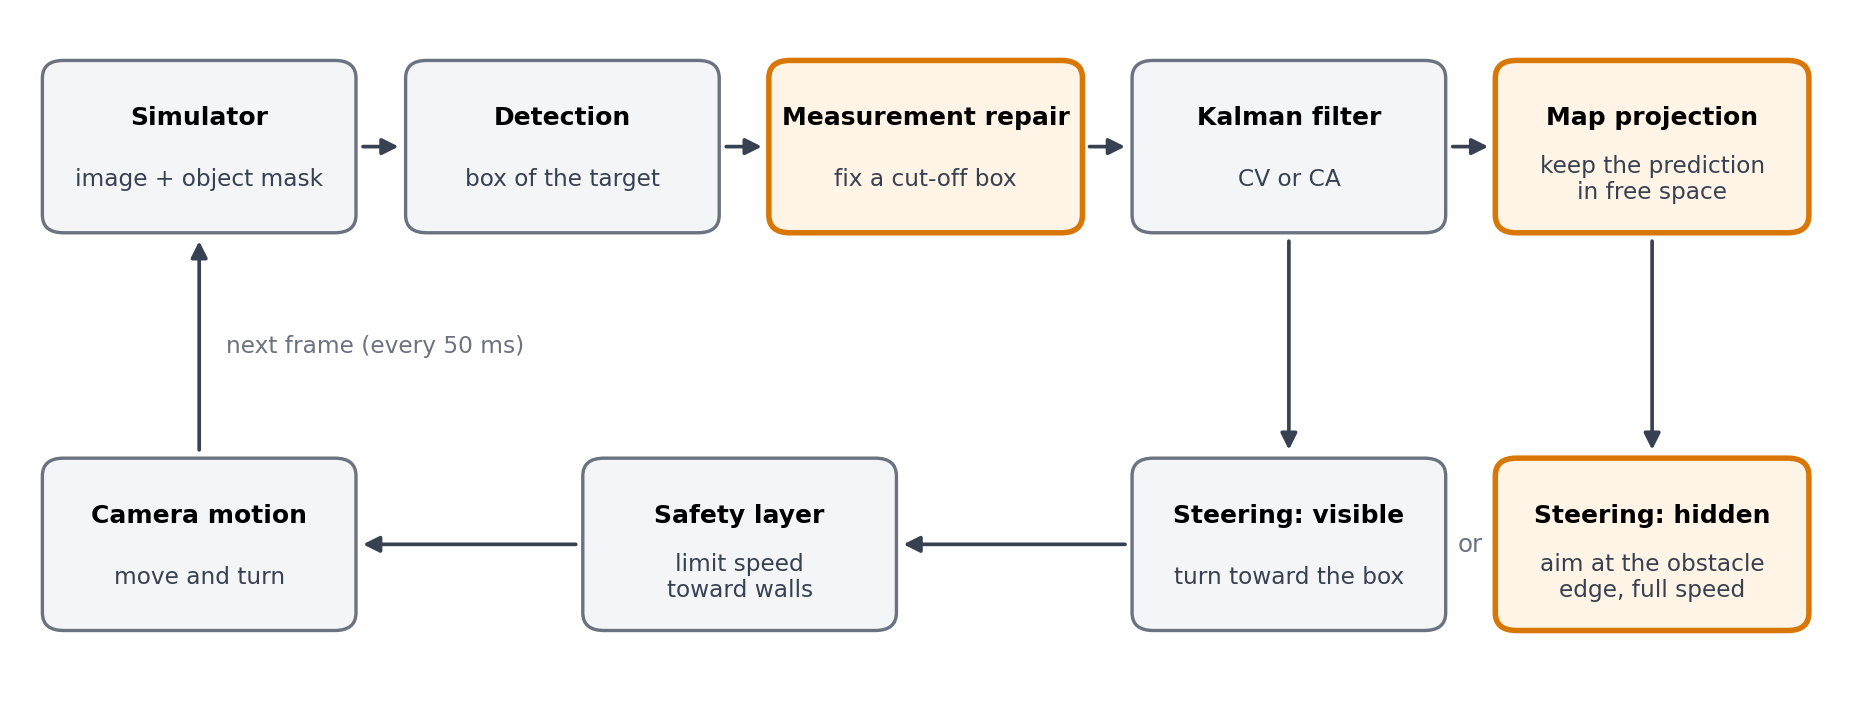
\includegraphics[width=15.5cm]{figs/fig_arch.png}
  \caption{One control step of the tracking system. Orange boxes are the parts added in this project: measurement repair and map projection form the MC-KF, and ``Steering: hidden'' is the edge-aiming rule used while the target is hidden.}
\end{figure}

\begin{table}[htbp]
  \centering
  \small
  \caption{Frozen benchmark configuration.}
  \renewcommand{\arraystretch}{1.15}
  \begin{tabular}{>{\raggedright\arraybackslash}p{0.247\linewidth}>{\raggedright\arraybackslash}p{0.295\linewidth}>{\raggedright\arraybackslash}p{0.368\linewidth}}
  \toprule
  \textbf{Item} & \textbf{Value} & \textbf{Reason} \\
  \midrule
  Corridor & W = 150 cm, walls 350 cm & Narrow indoor corridor \\
  Camera & 640$\times$480, hFOV 82.6\textdegree{}, pitch $-$15\textdegree{} & Tello spec; target centred at 250 cm \\
  Camera limits & v $\le$ 99 cm/s, |$\omega$| $\le$ 30\textdegree{}/s, acceleration $\le$ 200 cm/s\textsuperscript{2}, 20 Hz & Speed and rate from OA-VAT; turn-rate and acceleration limits set here \\
  Target & Person, 168 cm, speed 40–99 cm/s & Never faster than the camera \\
  Following distance & 250 cm & Optimum of the OA-VAT score \\
  Wall margin & camera $\ge$ 30 cm from walls & Near-clip limit 15 cm (measured) plus body radius and localisation slack \\
  \bottomrule
  \end{tabular}
\end{table}

\textbf{What is taken from OA-VAT.} Only the elements in Table 2 are inherited. Everything else is designed in this project: the track, camera setup, detector, controller, target behaviours, re-acquisition metric and the proposed architecture.

\begin{table}[htbp]
  \centering
  \small
  \caption{Elements inherited from OA-VAT.}
  \renewcommand{\arraystretch}{1.15}
  \begin{tabular}{>{\raggedright\arraybackslash}p{0.223\linewidth}>{\raggedright\arraybackslash}p{0.416\linewidth}>{\raggedright\arraybackslash}p{0.271\linewidth}}
  \toprule
  \textbf{Element} & \textbf{Inherited content} & \textbf{Difference in this project} \\
  \midrule
  Kalman filter & 8-D CV filter from the OA-VAT code (structure from DeepSORT \cite{r20}); noise weights 1/20 (position), 1/40 (velocity) & Used unchanged as the baseline; the CA filter extends it \\
  Evaluation protocol & Per-step score r = 1 $-$ |$\rho$ $-$ 250|/750 $-$ |$\theta$|/45; visible if $\rho$ $\le$ 750 cm and |$\theta$| $\le$ 45\textdegree{}; 500 steps; AR / EL / SR & Failure after 50 invisible steps (OA-VAT: after more than 50); r clipped to [$-$1, 1] before summing \\
  Control timing & 50 ms period (20 Hz), speed limit 99 cm/s, following distance 250 cm & None \\
  Simulator & gym-unrealcv FlexibleRoom scene and person model & Windows fixes; walls built from scripted blocks \\
  \bottomrule
  \end{tabular}
\end{table}

\textbf{Scope of the comparison.} Perception is simplified in the same way as control: detection uses the engine’s object mask instead of OA-VAT’s YOLOE, DINOv3 and ORTrack stack, and steps run in fixed 50 ms increments with no latency. OA-VAT’s own occlusion procedure is therefore not reproduced here. That procedure stops the camera, searches around the prediction with its detector for at most 15 frames, and then falls back to the planner. All results in this report compare configurations under the same detector and controller.


\subsection{Occlusion geometry}
A simple model is used to choose the following distance. The target turns the corner at a distance c from the inner corner, and the camera follows along the same path, a path length d behind; the target is treated as a point. When the target has walked a distance s past the corner, the wall blocks the view if $s^2 - d\,s + c\,d < 0$. This happens only if

\begin{equation}
  d > 4c
\end{equation}
and the target stays hidden over a path length

\begin{equation}
  L_{\mathrm{occ}} = \sqrt{d\,(d-4c)}
\end{equation}
With d = 250 cm and c = 40 cm this gives 150 cm (about 38 steps at 80 cm/s), which matches the engine's object mask. Each passage has a \emph{fade-out} phase, in which the wall gradually clips the box, followed by a \emph{fully blind} phase (Figure 2).
The model holds only when the camera follows the same path; a camera closer to the inner wall is blocked earlier, and one near the outer wall may not be blocked at all. It is therefore used only to choose d = 250 cm and c in [40, 60] cm; whether an episode contains an occlusion is measured from the object mask (Section 5.3).

\begin{figure}[H]
  \centering
  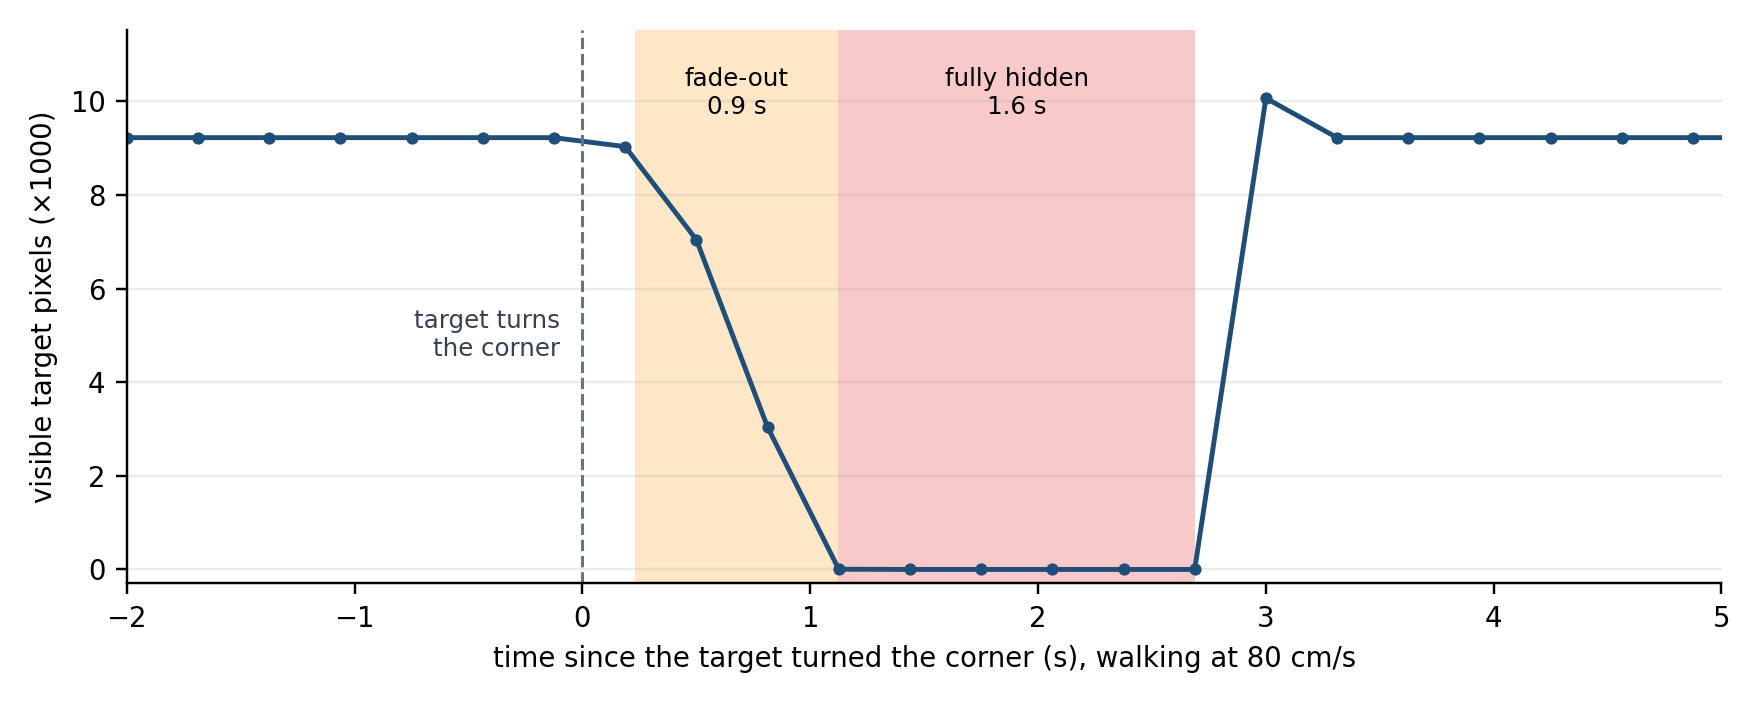
\includegraphics[width=14.5cm]{figs/fig_occlusion.png}
  \caption{Visible target pixels measured in the engine as the target walks around the corner (d = 250 cm, c = 40 cm, camera on the target's path, 80 cm/s). Shaded: the fade-out phase, in which the wall gradually cuts off the box, and the fully hidden phase.}
\end{figure}

\subsection{Target behaviour}
Each seed generates a random route through the corner and a random speed profile: every 2–4 s the target picks a new speed between 40 and 99 cm/s and changes to it with an acceleration of at most 80 cm/s\textsuperscript{2}. Nothing is tied to the corner, so the target may or may not change speed while it is hidden.

Because the route and speed are random, not every episode contains an occlusion, so the episodes fall into two groups, and results are reported for each:
\begin{itemize}
  \item \textbf{With occlusion} (36 of 40 seeds): the target is completely hidden for at least 5 frames. Only these episodes have a re-acquisition error.
  \item \textbf{Without occlusion} (4 of 40 seeds): the target is never completely hidden. These episodes check that the system does not harm ordinary tracking, using AR, SR and wall contacts.
\end{itemize}
The split is taken from the full system with CV; other configurations can differ by a few seeds, because their cameras follow slightly different paths.

\subsection{Baseline filter and controller}
\textbf{State.} The filter tracks the target's bounding box in the image. Its state is
\begin{equation}
  \mathbf{x} = [\,c_x,\ c_y,\ a,\ h,\ \dot c_x,\ \dot c_y,\ \dot a,\ \dot h\,]^{\top}
\end{equation}
and the measurement is the detected box $\mathbf{z} = [\,c_x,\ c_y,\ a,\ h\,]^{\top}$. Table 3 lists every entry, including the two added by the CA variant. One step is one frame (50 ms). The noise is scaled by the box height $h$, because a larger (closer) box also moves more in pixels.

\begin{table}[H]
  \centering
  \small
  \caption{Filter state entries and noise settings (standard deviations; the CV state has the first eight entries, the CA state all ten).}
  \renewcommand{\arraystretch}{1.15}
  \begin{tabular}{llllll}
  \toprule
  \textbf{Symbol} & \textbf{Meaning} & \textbf{Unit} & \textbf{Process noise} & \textbf{Measured (noise)} & \textbf{Used in} \\
  \midrule
  $c_x,\ c_y$ & box centre & px & $h/20$ & yes ($h/20$) & CV, CA \\
  $a$ & width-to-height ratio & -- & 0.01 & yes (0.1) & CV, CA \\
  $h$ & box height & px & $h/20$ & yes ($h/20$) & CV, CA \\
  $\dot c_x,\ \dot c_y$ & velocity of the centre & px/frame & $h/40$ & no & CV, CA \\
  $\dot a$ & change of the ratio & 1/frame & $10^{-5}$ & no & CV, CA \\
  $\dot h$ & change of the height & px/frame & $h/40$ & no & CV, CA \\
  $\ddot c_x,\ \ddot c_y$ & acceleration of the centre & px/frame\textsuperscript{2} & $h/800$ & no & CA only \\
  \bottomrule
  \end{tabular}
\end{table}

\textbf{Model.} The CV model assumes that the four velocities stay constant:
\begin{equation}
  \mathbf{x}_{k+1} = F\mathbf{x}_k + \mathbf{w}_k,\quad \mathbf{z}_k = H\mathbf{x}_k + \mathbf{v}_k,\quad F=\begin{bmatrix} I_4 & I_4\\ 0 & I_4\end{bmatrix},\quad H=\begin{bmatrix} I_4 & 0\end{bmatrix}
\end{equation}
so each position entry is advanced by its velocity, and only the box itself is measured.

\textbf{Baseline.} The baseline is this filter as released with OA-VAT (Table 2), with its original noise settings: it predicts every frame, updates whenever the target is detected, and coasts until the target reappears. Like every configuration, it runs with the safety layer of Section 5.6.

\textbf{CA variant.} The CA state adds the two accelerations of the box centre:
\begin{equation}
  \mathbf{x}_{\mathrm{CA}} = [\,c_x,\ c_y,\ a,\ h,\ \dot c_x,\ \dot c_y,\ \dot a,\ \dot h,\ \ddot c_x,\ \ddot c_y\,]^{\top}
\end{equation}
The box centre is advanced with both its velocity and its acceleration, while $a$ and $h$ keep the CV model. The accelerations are not measured; they are learned from how the box centre moves, and are limited to the pedestrian bound of 80 cm/s\textsuperscript{2}. Converted to pixels with the box height (a 168 cm person appears $h$ px tall) and one frame of 0.05 s, this gives
\begin{equation}
  |\ddot c_x|,\ |\ddot c_y| \le 80 \cdot \frac{h}{168} \cdot 0.05^2 \approx 0.0012\,h \ \ \text{px per frame}^2.
\end{equation}

\textbf{Controller.} When the target is visible, the camera turns toward the estimated bearing $\theta$ and keeps the estimated range $\hat\rho$ at 250 cm:
\begin{equation}
  \theta = \arctan\frac{c_x-320}{f_x},\qquad \hat{\rho} = \frac{f_x\cdot 168}{h}
\end{equation}
\begin{equation}
  \omega = \operatorname{clip}(3\theta,\ \pm 30^\circ/\mathrm{s}),\qquad v = \operatorname{clip}\big(2(\hat{\rho}-250),\ 0,\ 99\ \mathrm{cm/s}\big)
\end{equation}
Here 320 px is the image centre column, $f_x = 364.3$ px is the focal length, and 168 cm is the person's height, so $\hat\rho$ is the pinhole-camera range estimate. $\omega$ is the turn rate and $v$ the forward speed; the gains 3 and 2 were chosen by hand. In the baseline the same controller is also driven by the filter's prediction while the target is hidden, so the camera keeps steering toward the extrapolated box.

\subsection{Map-constrained Kalman filter (MC-KF)}
The MC-KF keeps the standard filter and adds two steps that use the map.

\textbf{Measurement repair (fade-out frames).} A frame counts as cut off when the target's pixel count falls below half of its peak over the last 8 fully visible frames. The occluding edge, projected from the map into the image, shows which side of the box is cut off. The centre is then rebuilt from the visible edge $u$ and the box width $w$ remembered from fully visible frames, $c_x = u \pm w/2$, and only $c_x$ is updated (Figure 3).

\begin{figure}[H]
  \centering
  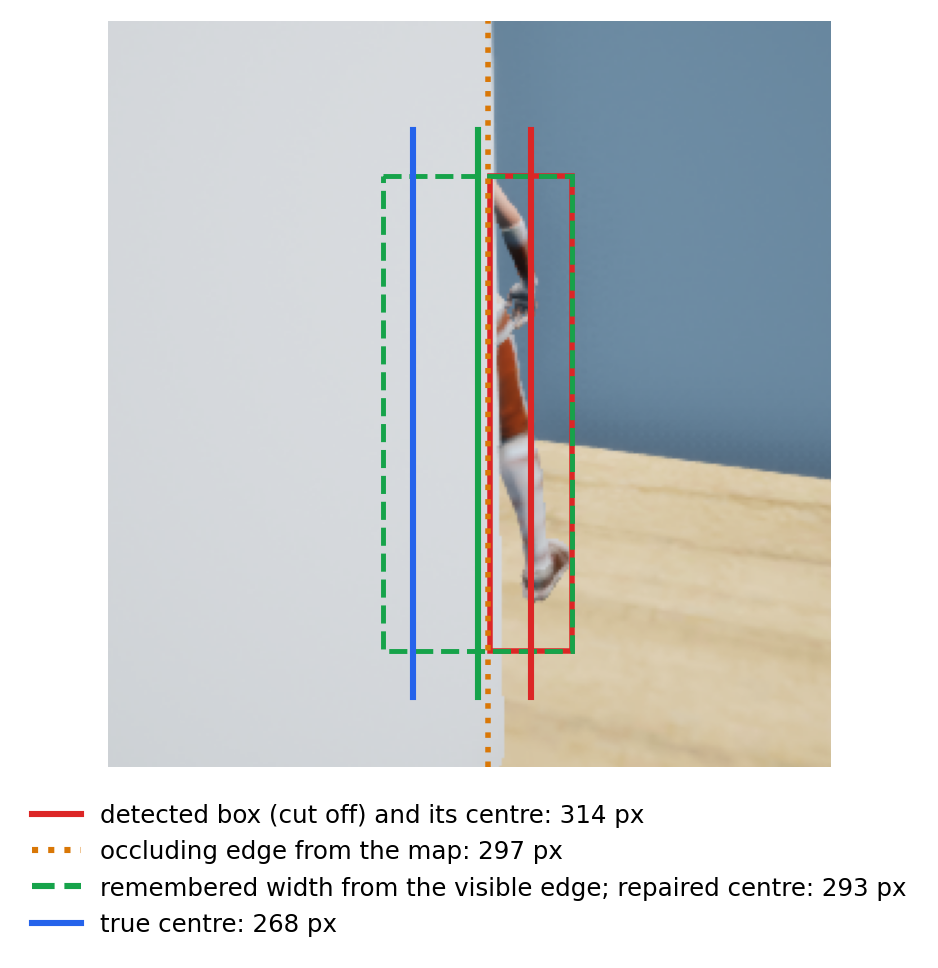
\includegraphics[width=10cm]{figs/fig_repair.png}
  \caption{Measurement repair on a real frame (camera view). Red: detected box and its centre; orange: occluding edge from the map; green: box rebuilt from the visible edge; blue: true centre. The error falls from 46 px to 25 px.}
\end{figure}

\textbf{Map projection (blind frames).} After each prediction, the predicted box is placed on the floor using the camera position $\mathbf{p}_{\mathrm{cam}}$, its heading $\psi$, and the bearing $\theta$ and range $\hat\rho$ from Section 5.4:
\begin{equation}
  \mathbf{p} = \mathbf{p}_{\mathrm{cam}} + \hat{\rho}\,\big[\cos(\psi+\theta),\ \sin(\psi+\theta)\big]^{\top}
\end{equation}
If $\mathbf{p}$ lies outside the free space, it is moved to the nearest free point and projected back into $(c_x, h)$. The covariance is not changed. This is estimate projection as described in \cite{r27} (Figure 4).

\begin{figure}[H]
  \centering
  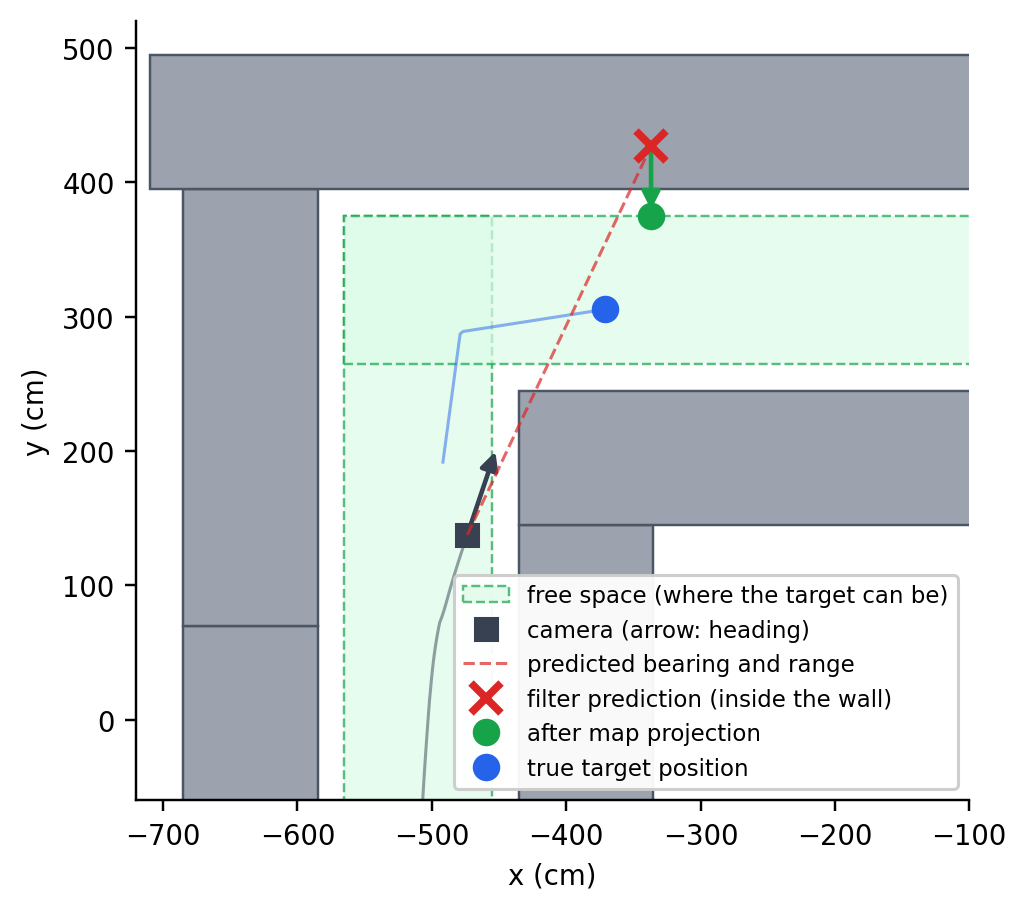
\includegraphics[width=10cm]{figs/fig_clamp.png}
  \caption{Map projection on the first blind frame of the same episode (top view). The prediction (red) lies inside the wall and is moved into the free space (green); its distance to the true position (blue) falls from 126 cm to 78 cm.}
\end{figure}

\subsection{Edge-aiming blind-phase control and safety}
\textbf{Edge aiming (fading and blind frames).} While the target is fading or hidden, the camera turns toward the image column of the occluding edge, because the target can only reappear past that edge, and its speed command is set to the maximum (99 cm/s). The filter's estimate (its \emph{belief}) is no longer used for steering. The filter keeps running: its prediction is compared with the target when it reappears, and it then continues with the new measurement. This simple rule is used because the test bench has no planner; in practice the camera slides along the wall toward the corner.

\textbf{Camera dynamics and safety layer.} The camera has inertia: its velocity is part of its state and can change by at most $A\,\Delta t$ per step, with $A = 200$ cm/s\textsuperscript{2} (a Tello-class drone) and $\Delta t = 0.05$ s, so it cannot stop instantly. Let $d_{\mathrm{wall}}$ be the camera's distance to the nearest wall and $u$ the part of its velocity that points toward that wall. The safety layer limits only this part, so that braking at the maximum deceleration from the next position always stops the camera before the 30 cm margin:
\begin{equation}
  u \le \sqrt{(A\Delta t)^2 + 2A\,(d_{\mathrm{wall}} - 30\,\mathrm{cm})} - A\Delta t
\end{equation}
This is the braking distance $u^2/2A$ written for discrete steps. The closer the camera is to the margin, the slower it may approach the wall, and at the margin it cannot approach at all; motion along the wall is not limited, and the heading is never changed. As a backup, if a step would still cross the margin, the movement toward the wall is cancelled and only the movement along the wall is kept. The safety layer is a prerequisite and is used in every configuration, including the baseline.

\subsection{Evaluation}
On a single corner the OA-VAT metrics (accumulated reward AR, episode length EL, success rate SR) change very little between methods, because every method eventually finds the target again. The main metric is therefore the \textbf{re-acquisition error}. When the target is detected again after at least 5 blind frames, it is the horizontal pixel distance between the filter’s predicted box centre and the centre of the newly detected box. All errors are reported in pixels, because the distance to the target at reappearance varies and a conversion to centimetres would be unreliable. Every configuration runs on the same 40 seeds (2000–2039) with identical target routes. Results are reported as paired differences, per-seed win counts and bootstrap 95\% confidence intervals.

\section{Progress Report and Revised Gantt Chart}
\subsection{Reproduction and motivating observations}
OA-VAT was reproduced on Windows with all three modules, including training the diffusion planner on 1,464 self-collected episodes. On UrbanCity the reproduction reached SR 0.95 and EL 487 (paper: 0.95 / 486), and on ParkingLot the planner raised SR from 0.70 to 0.90 (paper: 0.93). AR was 80–115 points lower than reported (270 vs 385 on UrbanCity, 314 vs 392 on ParkingLot). The reproduction is therefore close but not exact. It served to understand the method rather than to benchmark it.

Two observations from this stage, both with the full OA-VAT system, motivated the project. On an early four-corner test course (not the L-corner used later), target acceleration capped at the camera’s top speed reduced AR from 291 to 249 (10 episodes, one seed). In a ParkingLot variant where the target manoeuvres at corners, the confidence-aware predictor reached SR 0.85 against 0.90 without a predictor (20 episodes). Both samples are small, so these results are treated as motivation, not as evidence.

\subsection{The motion-model hypothesis}
The original plan was to replace CV with a stronger motion model. This was tested on the calibrated L-corner with 40 paired seeds of random target motion. With the inherited noise settings, CA and CV gave the same error (difference $-$2.0 px, 95\% CI [$-$6.4, 2.7]). With the measurement noise reduced to match the near-noiseless detector, the difference was still not significant ($-$3.8 px, CI [$-$7.7, 0.6]). Calibrating the noise itself helped a little (CV: 111.0 $\rightarrow$ 103.0 px). In most episodes the target did not change speed much while hidden: the median speed change during the blind phase was 5.3 cm/s, and only 9 of 36 episodes changed by more than 15 cm/s. The error therefore comes mainly from the estimate at the moment the target disappears, and a better motion model can do little about it.

\subsection{Measurement repair and steering during occlusion}
The next step was to correct the cut-off measurements. Early tests showed a side effect: when the camera still followed the filter's prediction, the corrected estimate led it too far behind the wall, so it missed the target reappearing at the corner.
Over 40 seeds without the map projection, measurement repair lowered the error by 72 px but lost the target in 3 episodes (SR 0.93).
With the projection, steering and flying by the prediction still gave 111 px more error than aiming at the edge at full speed (CI [93, 128]; worse on all 35 seeds; SR 0.97).
Edge aiming is therefore needed for measurement repair to pay off; together they gave the largest improvement in this study (Figure 5).

\begin{figure}[htbp]
  \centering
  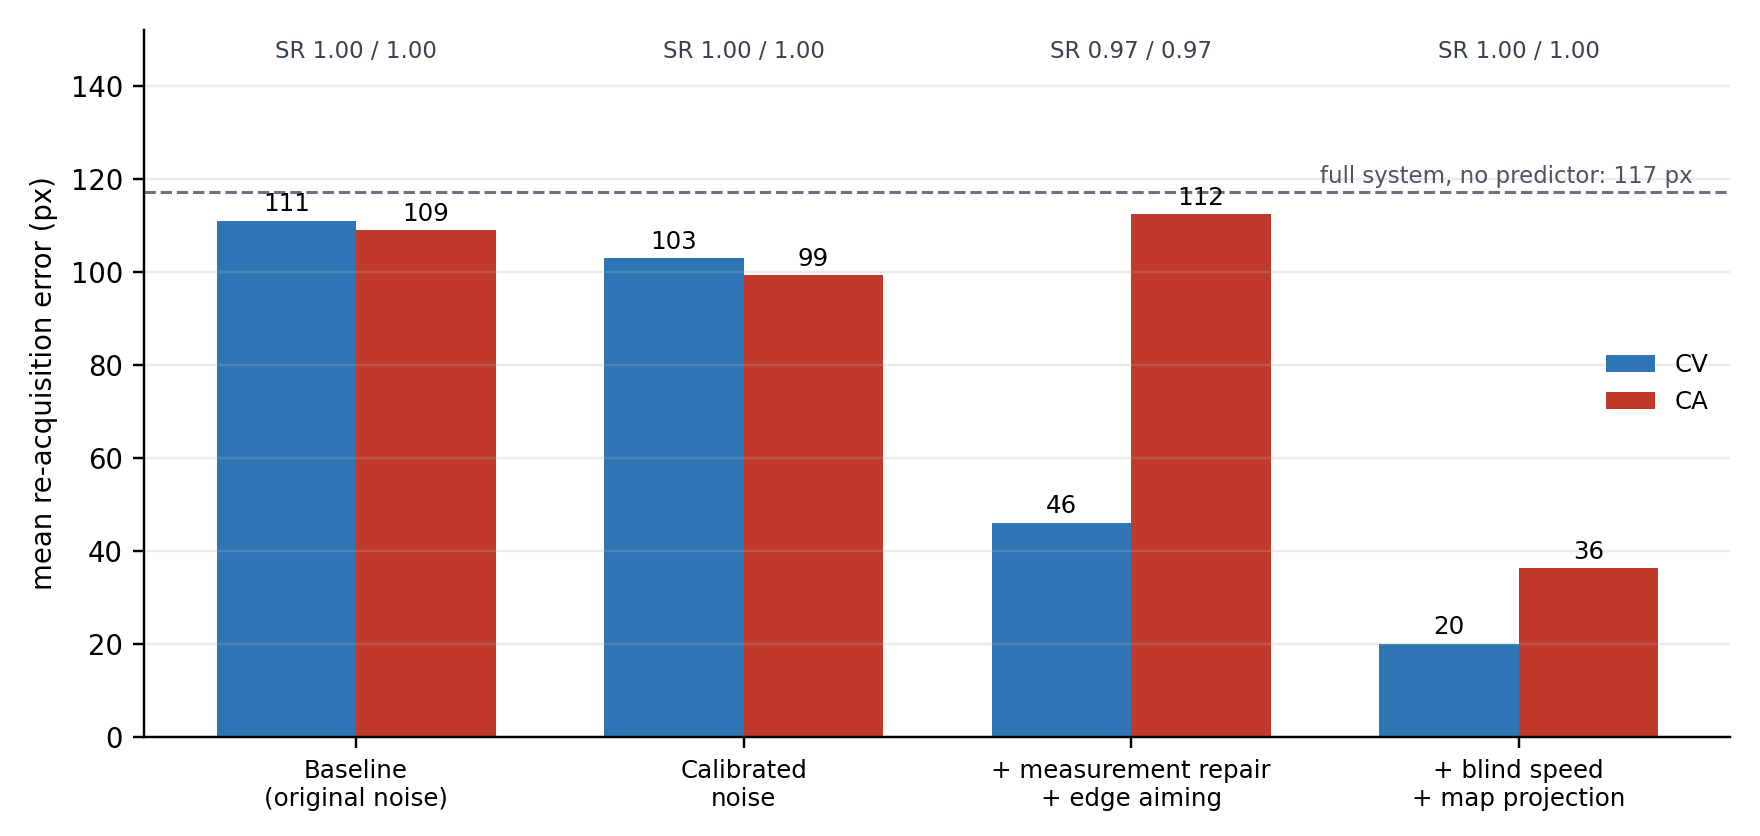
\includegraphics[width=14.5cm]{figs/fig_progress.png}
  \caption{Re-acquisition error at each development stage (random target motion, 40 paired seeds; all stages include the safety layer, and stages 2–4 use the calibrated measurement noise). SR is given above each pair of bars.}
\end{figure}

With CV, the error falls from 111.0 px (baseline) to 103.0 px (calibrated noise), 46.1 px (measurement repair and edge aiming) and 20.2 px (blind speed and map projection). With the original noise the full system reaches 21.0 px, so it does not depend on the calibration. CA is much worse than CV at the third stage (112 vs 46 px), likely because without the projection and the fixed blind speed its acceleration term carries the motion trend too far while the target is hidden.

\subsection{Current results}
\begin{table}[htbp]
  \centering
  \small
  \caption{Current results (random target motion, acceleration-limited camera, 40 seeds: 36 with occlusion, 4 without). All configurations include the safety layer; every episode succeeded (SR 1.00) and there were no wall contacts.}
  \renewcommand{\arraystretch}{1.15}
  \begin{tabular}{>{\raggedright\arraybackslash}p{0.40\linewidth}>{\raggedright\arraybackslash}p{0.17\linewidth}>{\raggedright\arraybackslash}p{0.15\linewidth}>{\raggedright\arraybackslash}p{0.15\linewidth}}
  \toprule
   & \multicolumn{2}{l}{\textbf{With occlusion}} & \textbf{Without occlusion} \\
  \textbf{Configuration} & \textbf{Re-acq. error (px)} & \textbf{AR} & \textbf{AR} \\
  \midrule
  Baseline: OA-VAT CV-KF (no map) & 111.0 & 453.3 & 460.1 \\
  Full system, no predictor & 117.2 & 455.9 & 460.9 \\
  \textbf{Full system, CV} & \textbf{21.0} & 455.7 & 461.1 \\
  Full system, CA & 34.2 & 455.7 & 461.1 \\
  \bottomrule
  \end{tabular}
\end{table}

The full system with CV lowers the re-acquisition error from 111.0 px to 21.0 px (paired difference $-$90 px, CI [$-$110, $-$70]; better on 34 of 36 seeds). Without a predictor the error is 117 px, so the Kalman filter is still needed. AR barely changes, because on one corner every configuration eventually finds the target.

\textbf{Why CA is worse.} The map projection is a fixed part of the system. While the target is hidden, a CV filter lags behind it, and the projection corrects this lag. A CA filter also corrects it with the acceleration it learned before the target disappeared, so together they over-correct: CA is 13 px worse than CV (CI [9, 17]; better on only 4 of 36 seeds). Setting the CA acceleration to zero during the blind phase removes most of this penalty (+2.8 px), and removing the projection makes CA as accurate as CV with the projection ($-$2.5 px, CI [$-$11, 6]). In this setting the improvement therefore comes from how the filter is used, not from the motion model.

\textbf{Ablations.} Table 5 removes one component at a time. Measurement repair matters most: without it the cut-off box enters the filter directly and the error exceeds that of using no predictor. Edge aiming lowers AR slightly, since the score rewards keeping the target centred, but improves re-acquisition. The safety layer is required and is removed only to show its effect: the camera, which cannot stop instantly, then hits walls and loses the target in 28\% of episodes.

\begin{table}[htbp]
  \centering
  \small
  \caption{Leave-one-out ablation, random target motion, acceleration-limited camera, 40 paired seeds (n.s. = confidence interval includes zero).}
  \renewcommand{\arraystretch}{1.15}
  \begin{tabular}{>{\raggedright\arraybackslash}p{0.34\linewidth}>{\raggedright\arraybackslash}p{0.26\linewidth}>{\raggedright\arraybackslash}p{0.30\linewidth}}
  \toprule
  \textbf{Removed from full system (CV)} & \textbf{$\Delta$ re-acq. error (px, 95\% CI)} & \textbf{Other effect} \\
  \midrule
  Measurement repair & +342 [+319, +366] & — \\
  Edge aiming & +58 [+45, +73] & AR +12 \\
  Fixed blind speed & +43 [+35, +52] & AR $-$26, SR 0.97 \\
  Map projection & +20 [+10, +30] & — \\
  Safety layer (required; removed only to show its effect) & +0.4 [$-$1.0, +2.0] (n.s.) & SR 0.72, AR $-$129, 122 wall contacts per episode \\
  \bottomrule
  \end{tabular}
\end{table}

\textbf{Limitations.} The results use an oracle detector and a single corner with a hand-coded map. They show the benefit of the system over the OA-VAT filter under identical conditions, not a head-to-head comparison with the full OA-VAT system, which would require both pipelines to run on the same real detector. With random motion, the target changed speed noticeably while hidden in only 9 of 36 episodes, so the results say more about occlusion in general than about speed changes in particular. Repeating a configuration gives small run-to-run differences, so only paired differences with confidence intervals are interpreted.

\subsection{Revised Gantt chart}
The original plan had five stages: a manoeuvring target, evidence that prediction degrades, CA/IMM baselines, a learned predictor, and a final comparison. The first three are done except for IMM. Because the gains came from how the filter is used rather than from the motion model, the MC-KF and edge aiming became the main focus and the learned predictor was dropped. Late in September all L-corner results were re-run with random target motion and camera inertia. The remaining weeks move the work to self-built mazes, where the first runs show that the simple edge-aiming rule is not enough, and add a planner to complete the system (Figure 6). The final report is due on 8 November 2026.

\begin{figure}[htbp]
  \centering
  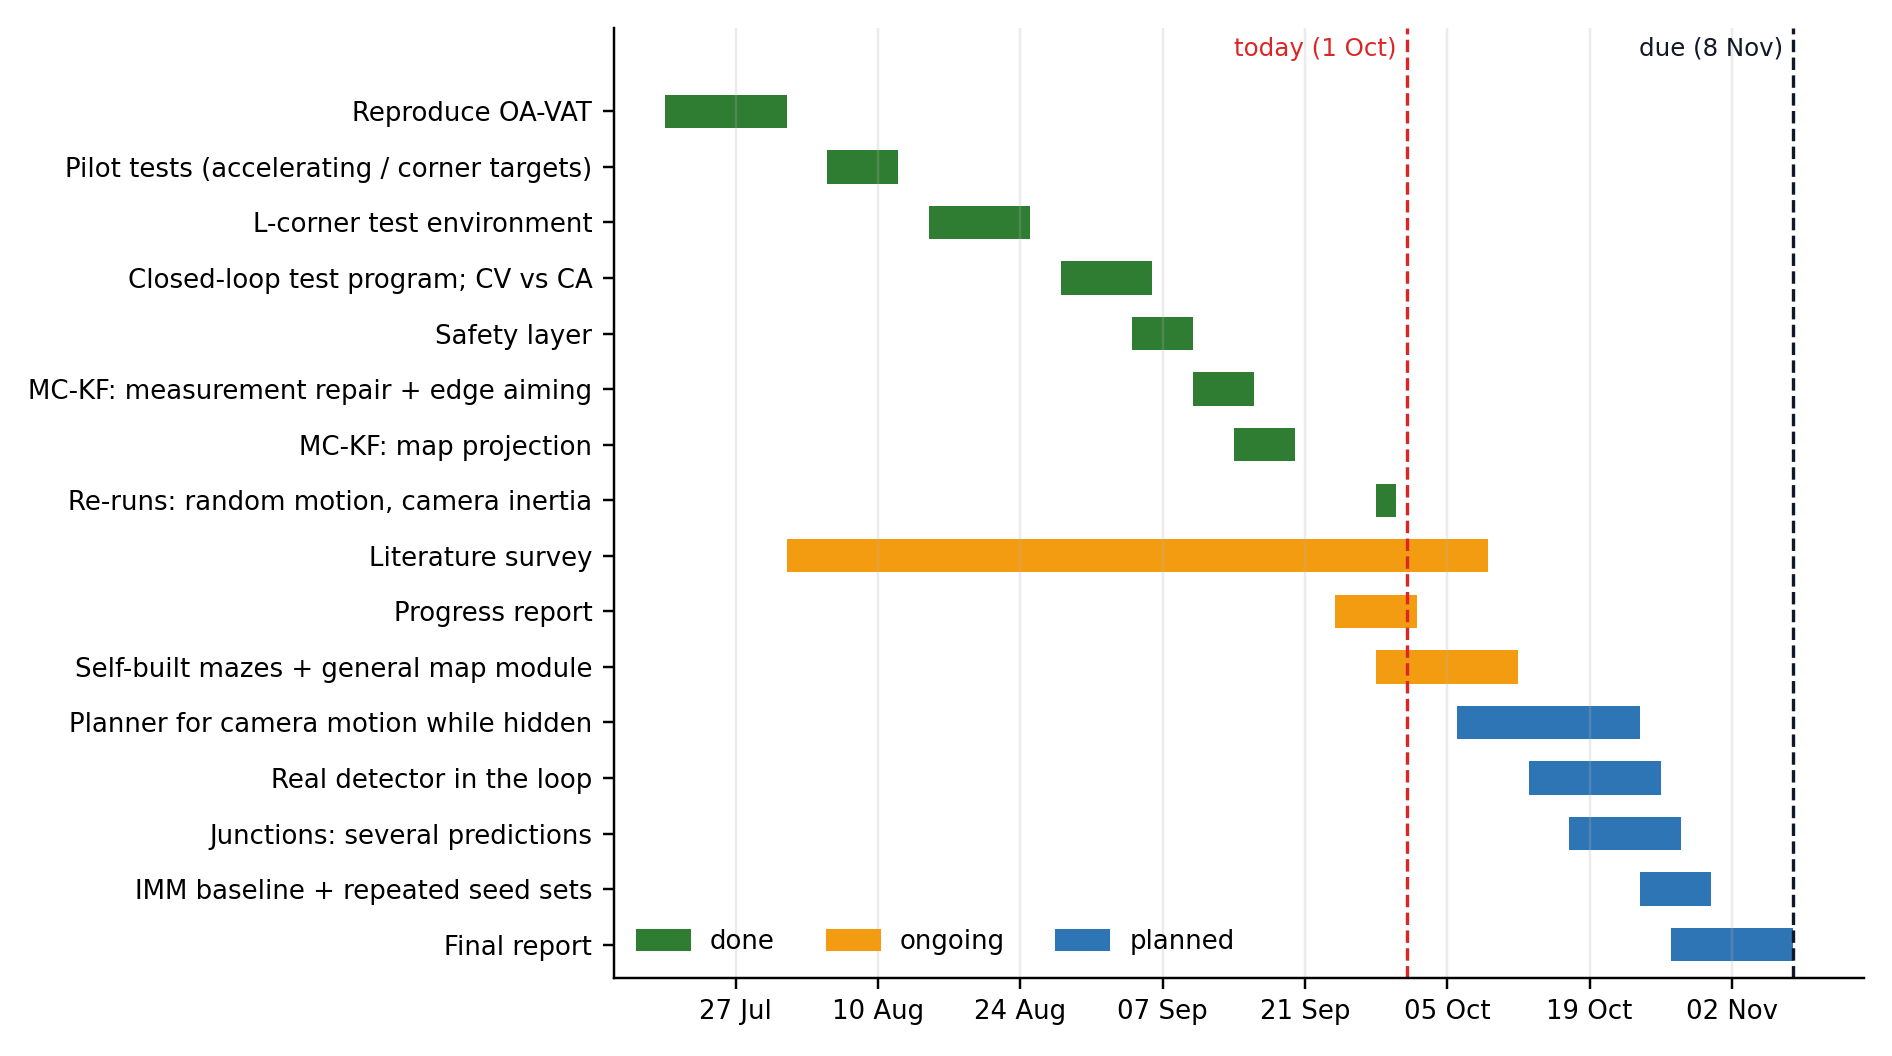
\includegraphics[width=15.5cm]{figs/fig_gantt.png}
  \caption{Revised Gantt chart (green: complete; orange: in progress; blue: planned).}
\end{figure}

\section{Planned Work}
The final report will add the following sections:

\begin{itemize}
  \item Self-built mazes and a general map module;
  \item A planner for camera motion while the target is hidden;
  \item Junctions with several possible exits;
  \item Real detector in the loop;
  \item Statistical validation and IMM baseline;
  \item Discussion and conclusion.
\end{itemize}
\clearpage
\begin{thebibliography}{99}
\addcontentsline{toc}{section}{References}
\bibitem{r1} W. Luo, P. Sun, F. Zhong, W. Liu, T. Zhang, and Y. Wang, ``End-to-end active object tracking via reinforcement learning,'' in \emph{Proc. Int. Conf. Machine Learning (ICML)}, 2018, pp. 3286–3295.
\bibitem{r2} W. Luo, P. Sun, F. Zhong, W. Liu, T. Zhang, and Y. Wang, ``End-to-end active object tracking and its real-world deployment via reinforcement learning,'' \emph{IEEE Trans. Pattern Anal. Mach. Intell.}, vol. 42, no. 6, pp. 1317–1332, 2020.
\bibitem{r3} H. Sun, K. Zhou, H. Gao, S. Zhang, J. Hu, X. Wen, Q. Ye, and M. Tan, ``Instance-level visual active tracking with occlusion-aware planning,'' arXiv:2604.21453, 2026.
\bibitem{r4} T. H. Chung, G. A. Hollinger, and V. Isler, ``Search and pursuit-evasion in mobile robotics: A survey,'' \emph{Autonomous Robots}, vol. 31, no. 4, pp. 299–316, 2011.
\bibitem{r5} W. Qiu, F. Zhong, Y. Zhang, S. Qiao, Z. Xiao, T. S. Kim, Y. Wang, and A. Yuille, ``UnrealCV: Virtual worlds for computer vision,'' in \emph{Proc. ACM Int. Conf. Multimedia}, 2017, pp. 1221–1224.
\bibitem{r6} F. Zhong, P. Sun, W. Luo, T. Yan, and Y. Wang, ``AD-VAT: An asymmetric dueling mechanism for learning visual active tracking,'' in \emph{Proc. Int. Conf. Learning Representations (ICLR)}, 2019.
\bibitem{r7} F. Zhong, P. Sun, W. Luo, T. Yan, and Y. Wang, ``Towards distraction-robust active visual tracking,'' in \emph{Proc. Int. Conf. Machine Learning (ICML)}, 2021, pp. 12782–12792.
\bibitem{r8} F. Zhong, X. Bi, Y. Zhang, W. Zhang, and Y. Wang, ``RSPT: Reconstruct surroundings and predict trajectory for generalizable active object tracking,'' in \emph{Proc. AAAI Conf. Artificial Intelligence}, 2023.
\bibitem{r9} F. Zhong, K. Wu, H. Ci, C. Wang, and H. Chen, ``Empowering embodied visual tracking with visual foundation models and offline RL,'' in \emph{Proc. European Conf. Computer Vision (ECCV)}, 2024.
\bibitem{r10} A. Wang, L. Liu, H. Chen, Z. Lin, J. Han, and G. Ding, ``YOLOE: Real-time seeing anything,'' in \emph{Proc. IEEE/CVF Int. Conf. Computer Vision (ICCV)}, 2025.
\bibitem{r11} O. Siméoni \emph{et al.}, ``DINOv3,'' arXiv:2508.10104, 2025.
\bibitem{r12} Y. Wu, X. Wang, X. Yang, M. Liu, D. Zeng, H. Ye, and S. Li, ``Learning occlusion-robust vision transformers for real-time UAV tracking,'' in \emph{Proc. IEEE/CVF Conf. Computer Vision and Pattern Recognition (CVPR)}, 2025, pp. 17103–17113.
\bibitem{r13} C. Chi, S. Feng, Y. Du, Z. Xu, E. Cousineau, B. Burchfiel, and S. Song, ``Diffusion policy: Visuomotor policy learning via action diffusion,'' in \emph{Proc. Robotics: Science and Systems (RSS)}, 2023.
\bibitem{r14} R. E. Kalman, ``A new approach to linear filtering and prediction problems,'' \emph{J. Basic Engineering}, vol. 82, no. 1, pp. 35–45, 1960.
\bibitem{r15} R. A. Singer, ``Estimating optimal tracking filter performance for manned maneuvering targets,'' \emph{IEEE Trans. Aerospace and Electronic Systems}, vol. AES-6, no. 4, pp. 473–483, 1970.
\bibitem{r16} X. R. Li and V. P. Jilkov, ``Survey of maneuvering target tracking. Part I: Dynamic models,'' \emph{IEEE Trans. Aerospace and Electronic Systems}, vol. 39, no. 4, pp. 1333–1364, 2003.
\bibitem{r17} H. A. P. Blom and Y. Bar-Shalom, ``The interacting multiple model algorithm for systems with Markovian switching coefficients,'' \emph{IEEE Trans. Automatic Control}, vol. 33, no. 8, pp. 780–783, 1988.
\bibitem{r18} Y. Bar-Shalom, X. R. Li, and T. Kirubarajan, \emph{Estimation with Applications to Tracking and Navigation}. New York: Wiley, 2001.
\bibitem{r19} A. Bewley, Z. Ge, L. Ott, F. Ramos, and B. Upcroft, ``Simple online and realtime tracking,'' in \emph{Proc. IEEE Int. Conf. Image Processing (ICIP)}, 2016, pp. 3464–3468.
\bibitem{r20} N. Wojke, A. Bewley, and D. Paulus, ``Simple online and realtime tracking with a deep association metric,'' in \emph{Proc. IEEE Int. Conf. Image Processing (ICIP)}, 2017, pp. 3645–3649.
\bibitem{r21} Y. Zhang \emph{et al.}, ``ByteTrack: Multi-object tracking by associating every detection box,'' in \emph{Proc. European Conf. Computer Vision (ECCV)}, 2022.
\bibitem{r22} J. Cao, J. Pang, X. Weng, R. Khirodkar, and K. Kitani, ``Observation-centric SORT: Rethinking SORT for robust multi-object tracking,'' in \emph{Proc. IEEE/CVF Conf. Computer Vision and Pattern Recognition (CVPR)}, 2023, pp. 9686–9696.
\bibitem{strongsort} Y. Du, Z. Zhao, Y. Song, Y. Zhao, F. Su, T. Gong, and H. Meng, ``StrongSORT: Make DeepSORT great again,'' \emph{IEEE Trans. Multimedia}, vol. 25, 2023.
\bibitem{amodal} Y. Zhu, Y. Tian, D. Metaxas, and P. Dollár, ``Semantic amodal segmentation,'' in \emph{Proc. IEEE Conf. Computer Vision and Pattern Recognition (CVPR)}, 2017.
\bibitem{r23} A. Rudenko, L. Palmieri, M. Herman, K. M. Kitani, D. M. Gavrila, and K. O. Arras, ``Human motion trajectory prediction: A survey,'' \emph{Int. J. Robotics Research}, vol. 39, no. 8, pp. 895–935, 2020.
\bibitem{r24} A. Alahi, K. Goel, V. Ramanathan, A. Robicquet, L. Fei-Fei, and S. Savarese, ``Social LSTM: Human trajectory prediction in crowded spaces,'' in \emph{Proc. IEEE Conf. Computer Vision and Pattern Recognition (CVPR)}, 2016, pp. 961–971.
\bibitem{r25} T. Salzmann, B. Ivanovic, P. Chakravarty, and M. Pavone, ``Trajectron++: Dynamically-feasible trajectory forecasting with heterogeneous data,'' in \emph{Proc. European Conf. Computer Vision (ECCV)}, 2020.
\bibitem{r26} K. M. Kitani, B. D. Ziebart, J. A. Bagnell, and M. Hebert, ``Activity forecasting,'' in \emph{Proc. European Conf. Computer Vision (ECCV)}, 2012.
\bibitem{r27} D. Simon, ``Kalman filtering with state constraints: A survey of linear and nonlinear algorithms,'' \emph{IET Control Theory \& Applications}, vol. 4, no. 8, pp. 1303–1318, 2010.
\bibitem{r28} T. Nägeli, J. Alonso-Mora, A. Domahidi, D. Rus, and O. Hilliges, ``Real-time motion planning for aerial videography with dynamic obstacle avoidance and viewpoint optimization,'' \emph{IEEE Robotics and Automation Letters}, vol. 2, no. 3, pp. 1696–1703, 2017.
\bibitem{r29} B. Penin, P. Robuffo Giordano, and F. Chaumette, ``Vision-based reactive planning for aggressive target tracking while avoiding collisions and occlusions,'' \emph{IEEE Robotics and Automation Letters}, vol. 3, no. 4, pp. 3725–3732, 2018.
\bibitem{r30} R. Bonatti, W. Wang, C. Ho, A. Ahuja, M. Gschwindt, E. Camci, E. Kayacan, S. Choudhury, and S. Scherer, ``Autonomous aerial cinematography in unstructured environments with learned artistic decision-making,'' \emph{J. Field Robotics}, vol. 37, no. 4, pp. 606–641, 2020.
\bibitem{r31} Z. Han, R. Zhang, N. Pan, C. Xu, and F. Gao, ``Fast-Tracker: A robust aerial system for tracking agile target in cluttered environments,'' in \emph{Proc. IEEE Int. Conf. Robotics and Automation (ICRA)}, 2021, pp. 328–334.
\bibitem{r32} J. Ji, N. Pan, C. Xu, and F. Gao, ``Elastic Tracker: A spatio-temporal trajectory planner for flexible aerial tracking,'' in \emph{Proc. IEEE Int. Conf. Robotics and Automation (ICRA)}, 2022.
\bibitem{r33} H. Oleynikova, Z. Taylor, M. Fehr, R. Siegwart, and J. Nieto, ``Voxblox: Incremental 3D Euclidean signed distance fields for on-board MAV planning,'' in \emph{Proc. IEEE/RSJ Int. Conf. Intelligent Robots and Systems (IROS)}, 2017.
\bibitem{r34} A. D. Ames, S. Coogan, M. Egerstedt, G. Notomista, K. Sreenath, and P. Tabuada, ``Control barrier functions: Theory and applications,'' in \emph{Proc. European Control Conf. (ECC)}, 2019, pp. 3420–3431.
\end{thebibliography}

\end{document}
